
The calibration consortium was formed in November 2018 as a joint single and dual phase consortium, with a consortium leader and a technical leader. Figure~\ref{fig:orgchart} shows the organization of the consortium. The calibration consortium board currently comprises institutional representatives from 11 institutions as shown in Table~\ref{tab:gen-calib-org}. The consortium leader is the spokesperson for the consortium and responsible for the overall scientific program and management of the group. The technical leader of the consortium is responsible for managing the project for the group. 

The consortium's initial mandate is the design and prototyping of a laser calibration system, a neutron generator, and possibly a radioactive source system, so the consortium is organized into three working groups, each dedicated to one system. Each group has a designated working group leader.
%The \dword{tdr} editors are responsible for the overall editing and delivery of the \dword{tdr} document.


\begin{dunefigure}[Organizational chart for the calibration consortium]{fig:orgchart}
{Organizational chart for the calibration consortium.}
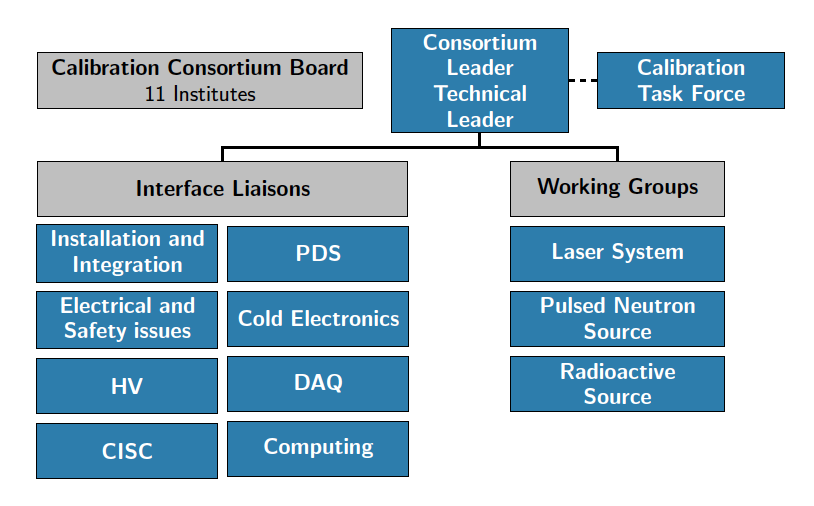
\includegraphics[height=3.0in]{graphics/orgchart_calib_sp.png}
\end{dunefigure}


\begin{dunetable}
[Calibration consortium institutions]
{lc}
{tab:gen-calib-org}
{Current Calibration Consortium Board Institutional Members and Countries.}
Member Institute     &  Country       \\
LIP & Portugal \\ \colhline
University of Bern (Bern) & Switzerland \\ \colhline
Los Alamos National Lab (LANL) & USA \\ \colhline
Michigan State University (MSU) & USA \\ \colhline
Colorado State University (CSU) & USA \\ \colhline
University of Iowa & USA \\ \colhline
University of Hawaii (Hawaii) & USA \\ \colhline
University of Pittsburgh (Pitt) & USA \\ \colhline
Boston University (BU) & USA \\ \colhline
University of California, Davis (UC Davis)& USA \\ \colhline
South Dakota School of Mines and Technology (SDSMT) & USA \\ 
\end{dunetable}

In addition, Figure~\ref{fig:orgchart} shows several liaison roles currently being established 
%\todo{These are being established after we have had initial interfaces and critical issues clarified} 
to facilitate connections with other groups and activities:
\begin{itemize}
    \item Detector integration and installation,
    \item Electrical and safety issues,
    \item \dword{daq},
    \item Computing,
    \item Cryogenic instrumentation and slow controls (CISC),
    \item Cold electronics,
    \item High voltage,
    \item Photon Detection System.
\end{itemize}

%\fixme{KM adjusted above from "planned" to state will exist by Summer 2019}

Currently, new institutions are added to the consortium  following an expression of interest from the interested institute and upon obtaining consensus from the current consortium board members.

%if the consortium board members agree, new members are added from other institutions if the new institutions express an interest through a petition to the board.